
\section{Image vs. Textual Screen Representation} \label{sec:img_vs_text}
Most ACUs either use image or text observations, or a combination of them.
In the following, we provide a comparison between image and textual screen observations.
In \cref{fig:text-repr-advantages}, we illustrate that textual screen representations offer unique strengths, particularly in exposing hidden semantics and structural relationships.
However, these strengths are often undermined by practical drawbacks (see \cref{fig:text-repr-disadvantages}), such as verbosity and inconsistency, especially when deployed in real-world environments.
These findings are in line with the works of \cite{he_actionbert_2021,wang_enabling_2023,li_zero-shot_2023,zheng_gpt-4vision_2024,cheng_seeclick_2024} and can be summarized as follows:
%
\begin{figure}[htbp]
\centering
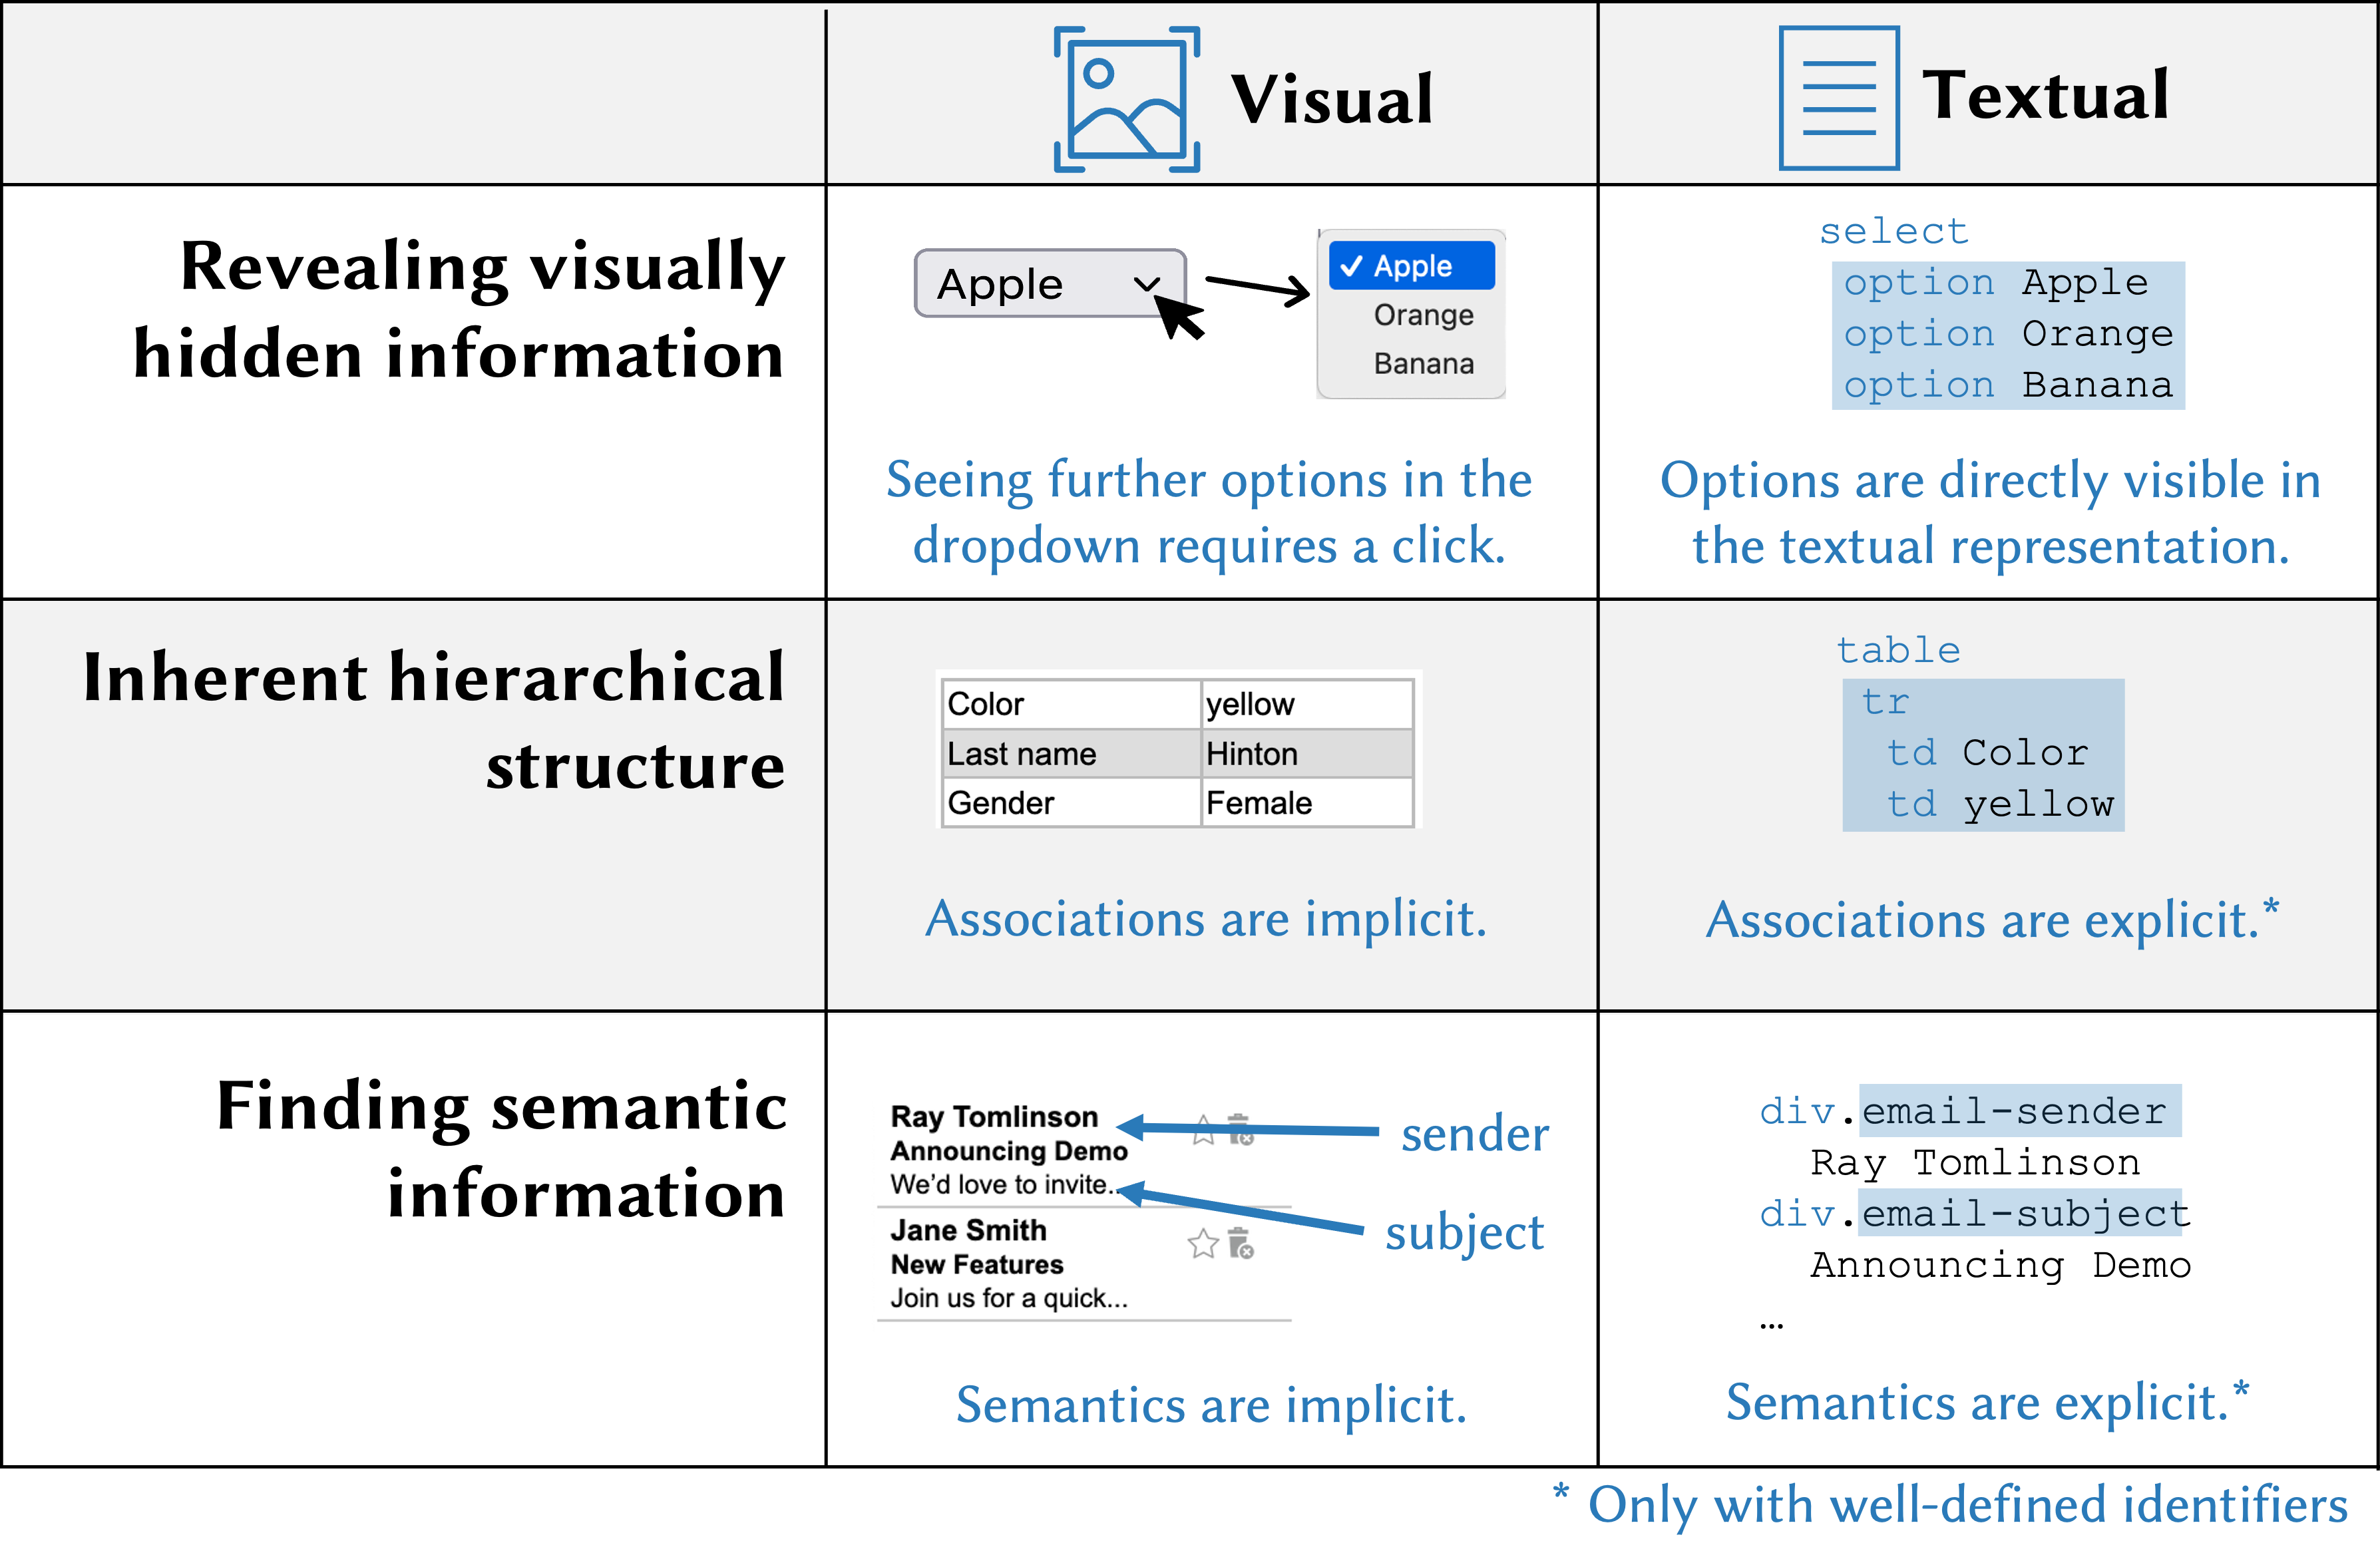
\includegraphics[width=0.6\linewidth]{figures/text_repr_advantages.png}
\caption{Advantages of textual screen representations.}
\Description{
The figure compares visual and textual interfaces across three axes. 
1. Revealing visually hidden information: Textual representation displays all dropdown options directly in code, unlike the visual interface, which requires user interaction. 
2. Inherent hierarchical structure: Textual HTML code explicitly defines structure using tags like <table>, <tr>, and <td>, while visual layouts only imply structure. 
3. Finding semantic information: Textual markup contains identifiers like ``email-sender'' and ``email-subject'', whereas visual cues are inferred from layout and formatting.
}
\label{fig:text-repr-advantages}
\end{figure}
%
\begin{figure}[htbp]
\centering
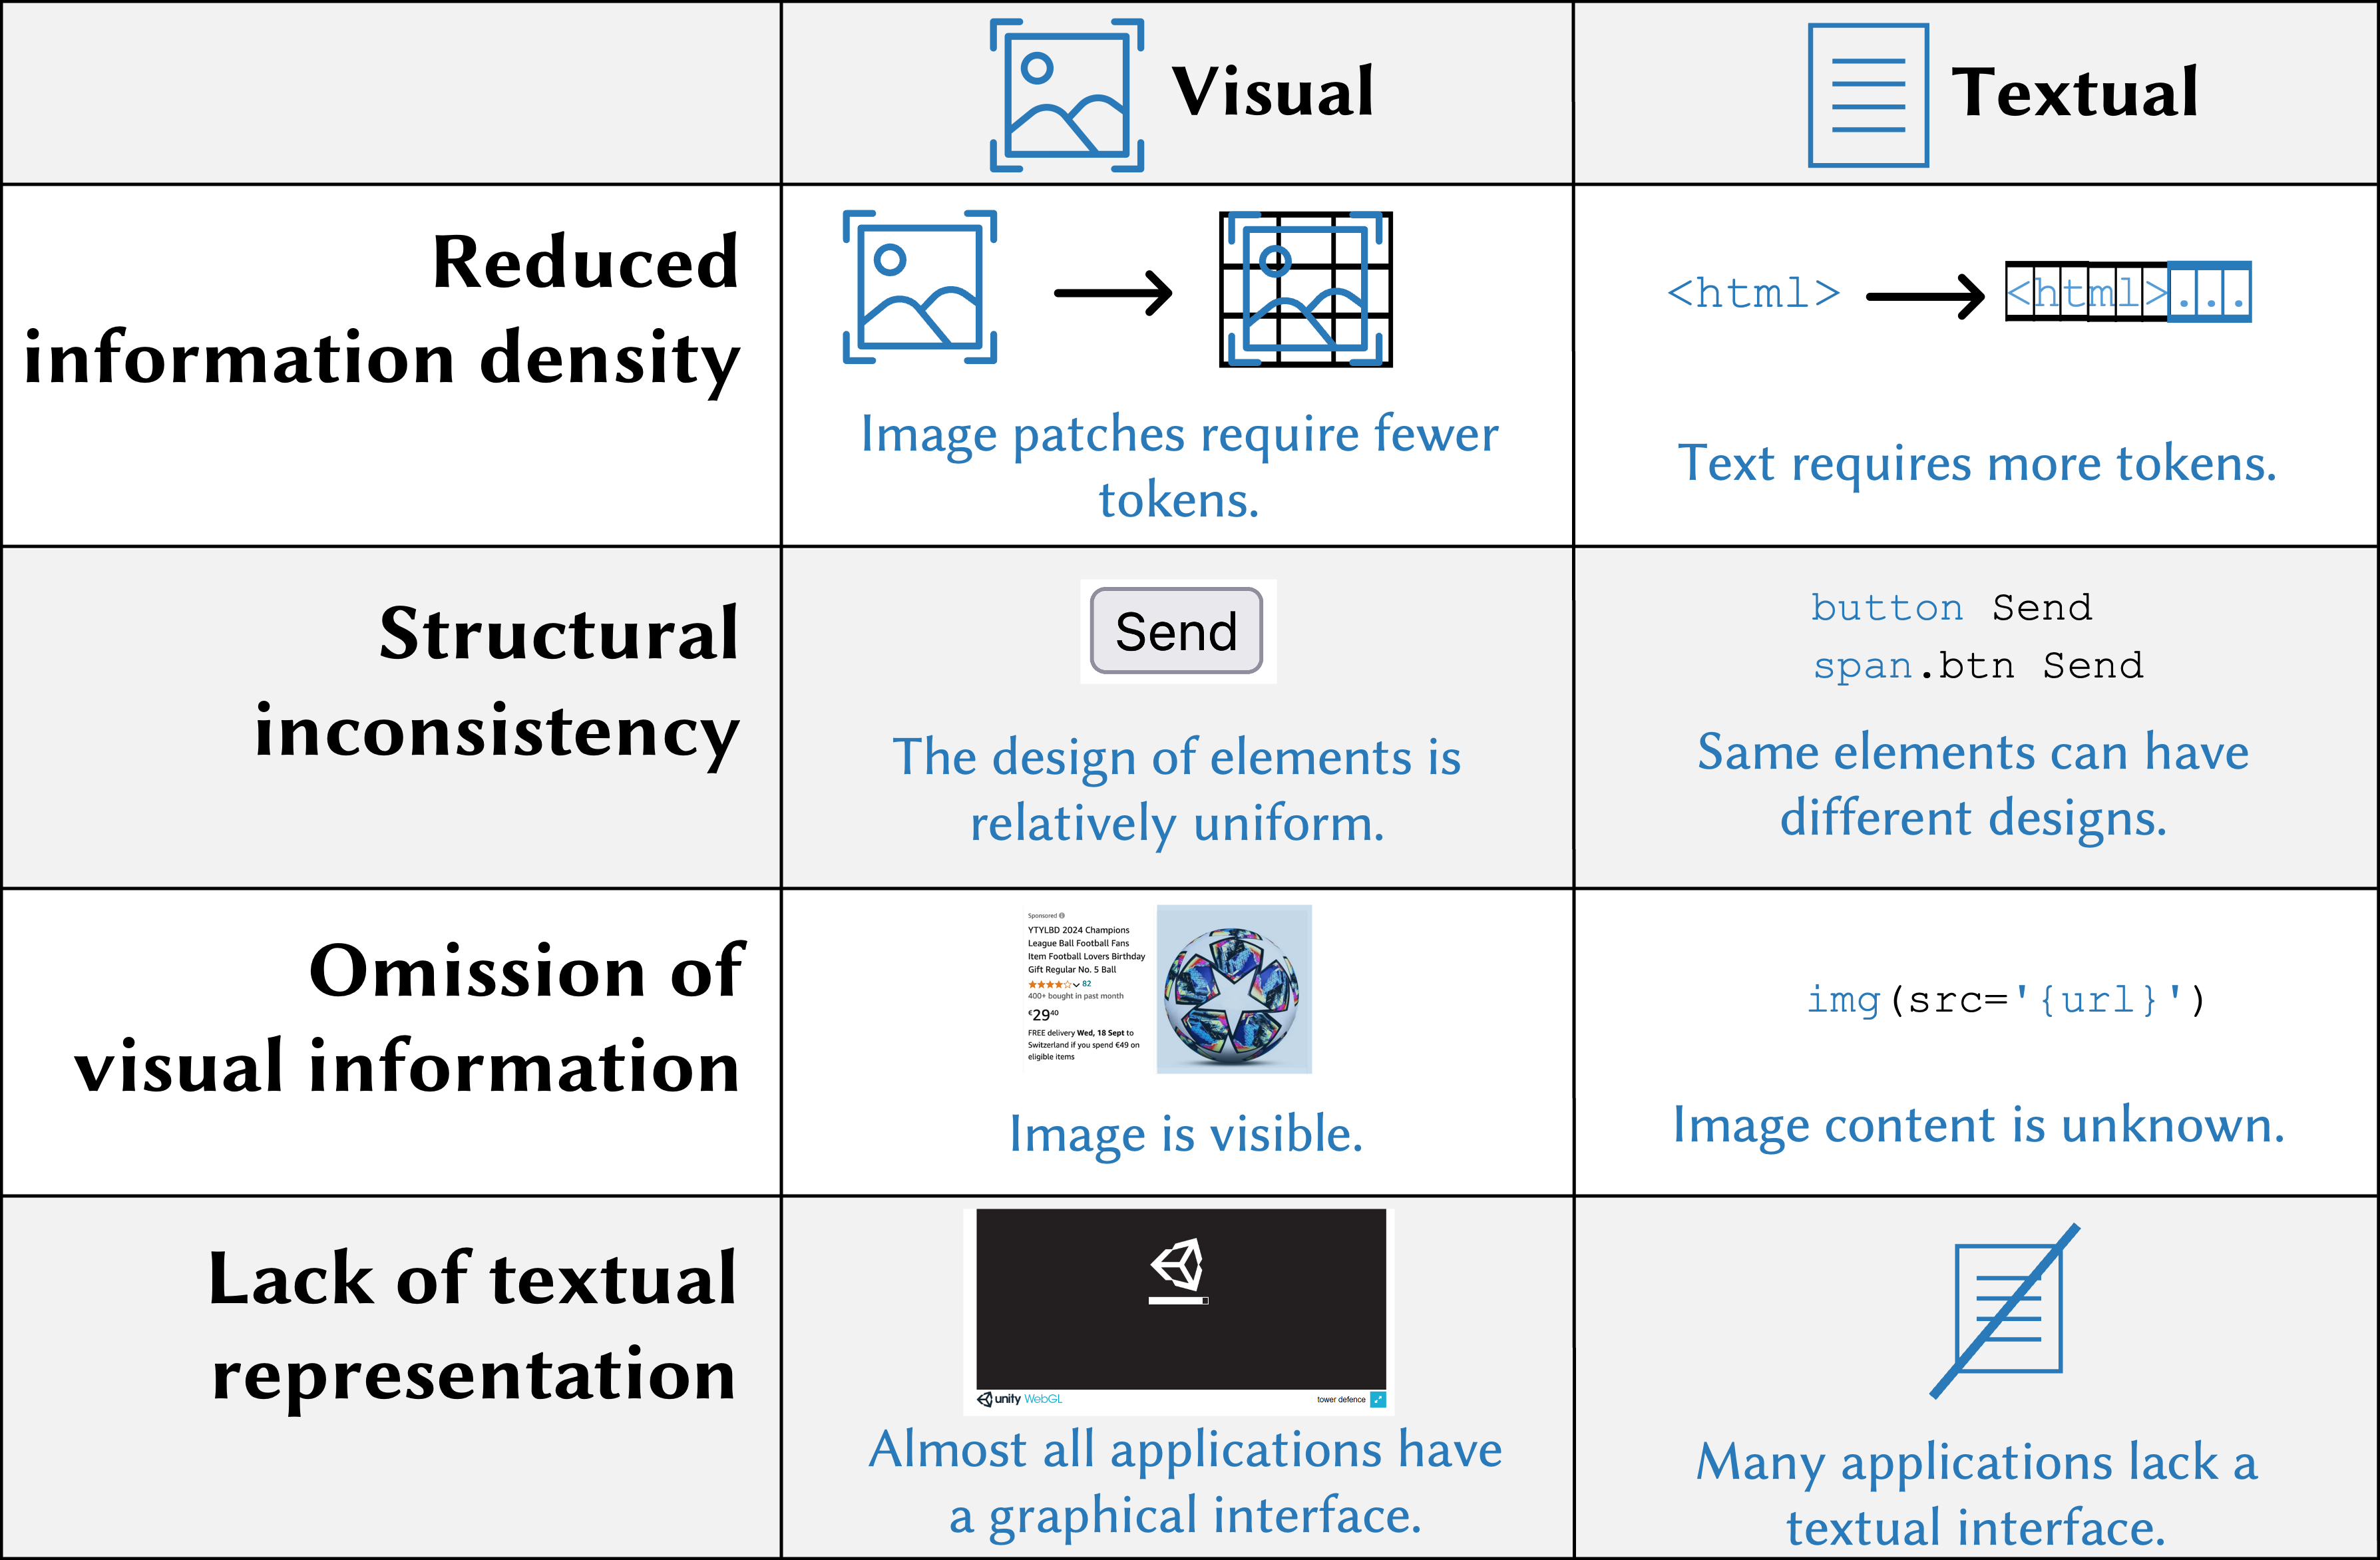
\includegraphics[width=0.6\linewidth]{figures/text_repr_disadvantages.png}
\caption{Disadvantages of textual screen representations.}
\Description{
The figure compares limitations of visual and textual representations across four categories.
1. Reduced information density: Visual image patches can represent more with fewer tokens than textual equivalents.
2. Structural inconsistency: In HTML, the same function (e.g., a button) may be represented differently across applications, whereas in visuals, the rendering is relatively uniform.
3. Omission of visual information: Textual code like img(src='{url}') lacks embedded image content, while visuals show actual images.
4. Lack of textual representation: Some applications only have visual interfaces with no textual HTML representation.
}
\label{fig:text-repr-disadvantages}
\end{figure}
%
\begin{description}
    \item[Advantages] of textual screen representations are: \hfill
    \begin{description}
        \item[Revealing visually hidden information:] 
            Textual representations can explicitly show information that may be visually hidden in images, such as items within a collapsed drop-down menu.
        \item[Inherent hierarchical structure:] 
            Textual representations, like the Document Object Model (DOM) tree, are structured in a hierarchical tree, facilitating a clearer understanding of relationships between elements \citepeg{jia_dom-q-net_2019}.
        \item[Explicit semantic information:] 
            Textual representations often include semantic information in element attributes that are not visible in images, such as \texttt{id} tags. For example, the \texttt{id} attribute in \texttt{\(<\)input id="flight-from"\(>\)} indicates that the input field corresponds to the flight departure location (example taken from the MiniWoB++ benchmark \citep{shi_world_2017}).
    \end{description}
    \item[Disadvantages] of textual screen representations are: \hfill
    \begin{description}
        \item[Reduced information density:] 
            Some text formats, particularly raw HTML, can introduce verbosity that reduces the overall information density.
        \item[Structural inconsistency:] 
            Visually similar content can be rendered using different underlying structures. For example, a button might be implemented with either a \texttt{<button>} or a \texttt{<span>} tag. Similarly, visually similar components can have vastly different underlying code due to different implementation choices, such as the selected styling framework (e.g., Bootstrap\footnote{\url{https://getbootstrap.com/}} vs. Tailwind CSS\footnote{\url{https://tailwindcss.com/}}) and HTML-generating framework (e.g., Angular\footnote{\url{https://angular.dev/}} vs. React\footnote{\url{https://react.dev/}}).
        \item[Omission of visual information:] 
            Textual representations often lack information about spatial relationships and positioning that can be critical in understanding the screen's layout.
        \item[Lack of textual representation:] 
            Some screen components, such as embedded plugins, may not have an alternative textual screen representation. Certain applications may entirely lack any alternative textual screen representation.
    \end{description}
\end{description}

Some of these disadvantages can be mitigated through engineering solutions. For instance, the absence of visual positioning can be addressed by incorporating absolute or relative screen coordinates into the textual screen representation \citepeg{shi_world_2017, liu_reinforcement_2018}, or by embedding elements with information from nearby neighboring elements \citep{liu_reinforcement_2018}. 
Additionally, the verbosity inherent in raw text can be reduced by simplifying the observations $o_t \rightarrow o_t^*$.
However, these mitigation strategies usually do not fully overcome the inherent limitations observed in practice.


\section{Code Generation Example} \label{sec:code_generation_examples}

As illustrated in Figure~\ref{fig:action-space-code}, executable code actions generated by agents can vary significantly in both structural complexity and abstraction level. Specifically, we distinguish between straight-line execution versus control-flow logic, and the use of task-tailored APIs versus general-purpose APIs. 

\begin{figure}[htbp]
    \centering
    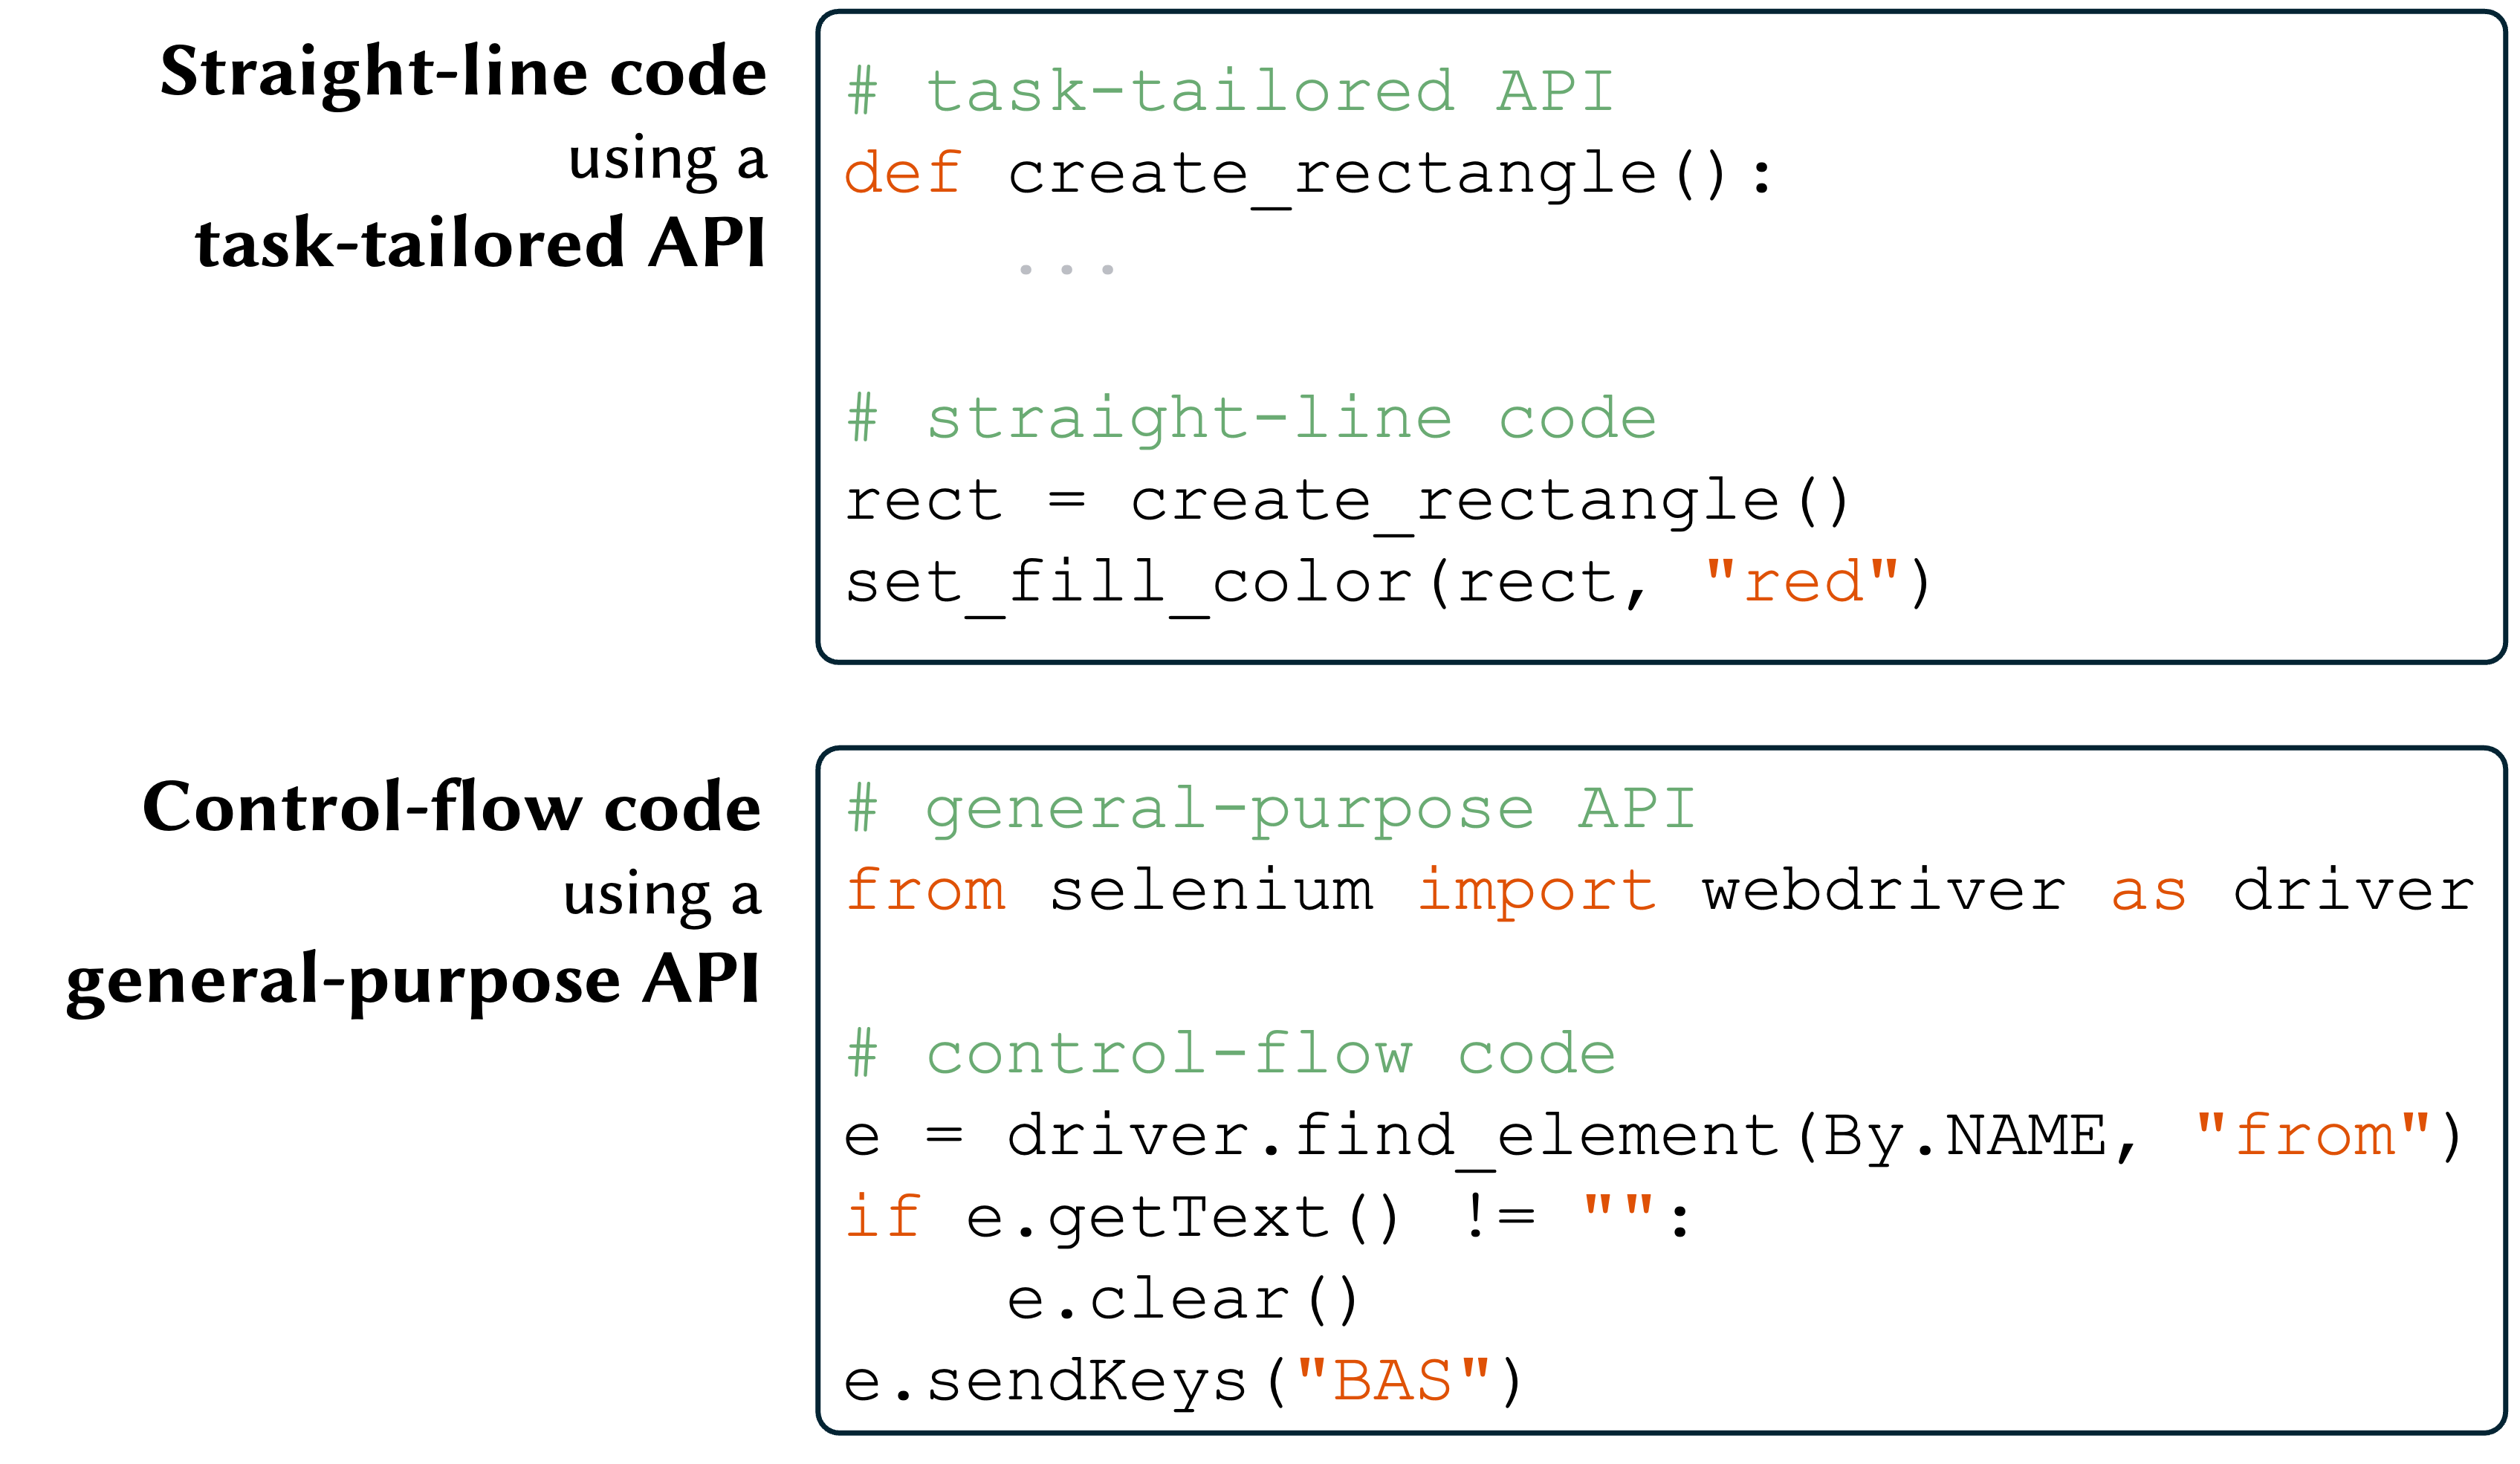
\includegraphics[width=0.6\linewidth]{figures/action_space_code.png}
    \caption{Two examples of executable Python code actions. Two different structures (straight-line or with control flow) and API abstraction levels (task-tailored or general-purpose) are shown.}
    \Description{
    The image compares two coding paradigms: straight-line code using a task-tailored API, and control-flow code using a general-purpose API.
    The top half shows straight-line code for a graphics task using a task-specific API. The function \texttt{create\_rectangle} is defined and then invoked, followed by setting the fill color to red using \texttt{set\_fill\_color}. The code has a custom function and is sequential.
    The bottom half shows control-flow code using Selenium, a general-purpose web automation library. It imports the webdriver, finds an element by its name attribute, checks if the element contains text, clears it if so, and then sends keys ``BAS'' to the element. The code includes an explicit if-statement and imports a library function, demonstrating more complex logic.
    }
    \label{fig:action-space-code}
\end{figure}

